% !TEX root = 00_arbeit.tex


%---------------------------------------------------------------------------------
%% Algorithmen

\section{Herleitung und Vergleich des Backpropagation und Levenberg-Marquardt Algorithmus}\label{sec:algorithm}

Im \autoref{sec:ANN-Modelle} wurden Modelle künstlicher neuronaler Netze verschiedener Kategorien vorgestellt, stärken sowie schwächen aufgezeigt und in mögliche Anwendungsgebiete eingeteilt. In \autoref{sec:strompreis} wurden die spezifischen Eigenschaften von Strompreisen aufgeführt und Modelle genannt die zur Vorhersage eingesetzt wurden. Vor dem Hintergrund der Beiden Kapitel erfolgt in diesem Abschnitt die Vorstellung der am häufigsten eingesetzten Algorithmen. Aus \autoref{sec:literaturueberblick} ist zu entnehmen, dass zur Modellierung und Vorhersage von Strompreisen das MLP das am meisten genutzte Netzwerk ist. Darüber hinaus wird das Backpropagation gefolgt vom Levenberg-Marquardt Lernalgorythmus am häufigsten eingesetzt. In diesem Abschnitt werden beide Algorithmen hergeleitet und vorgestellt. Anschließend werden die Vorzüge bzw. die Nachteile diskutiert. 

\subsection{Gemeinsame Grundlage}
Für beide Algorithmen wird wie bereits zu beginn des Abschnittes erwähnt das MLP-Netz benutzt. Das zu betrachtende Netzwerk besteht aus $(X_{i}, i=1,\dots,I)$ Eingabeneuronen, gefolgt von $(Z_{h}, h=1,\dots,H)$ verdeckten Neuronen und schließlich $(Y_{o}, o=1,\dots,O)$ Ausgabeneuronen. Hieraus ergeben sich drei Schichten an Neuronen und zwei Schichten an trainierbaren Gewichten $w_{hi}$ und $w_{oh}$. Zusätzlich sind die Aktivierungsfunktionen aller Neuronen gleich und Differenzierbar. In \autoref{fig:MLP-Algorithm} ist das betrachtete Netzwerk abgebildet.

\begin{figure}[!htb]
    \centering
    %---------------------------------------------------------------
        %% MLP-Algorithm
        %-----------------------------------------
            %---------------------------------------------------------------
        %% MLP-Algorithm
        %-----------------------------------------
\begin{tikzpicture}[>=stealth', node distance=\layersep cm, shorten >=1pt]
        \def\layersep{1.8}            % vertikal distance between the layers
        \def\neuronsep{1.8}         % Horizontal distance between neurons
        \def\dlsize{2}            % distance between node and layer lable
        \def\inout{\layersep*.65}   % Size of in- and output-arrow
        \def\siz{.8}                % neuronsize
        \def\y{5}                   % Start of the most upper layer
        \def\ni{2}                  % Amount of input neurons
        \def\nh{3}                  % Amount of hidden neurons
        \def\no{2}                  % Amount of output neurons
        \tikzstyle{neuron}=[circle,draw=black,minimum size=\siz cm,inner sep=2pt]
        \tikzstyle{annot} = [text width=6em, text centered]
        \tikzset{fontscale/.style = {font={\fontsize{#1pt}{#1pt}\selectfont}}}

        \newcommand{\neurono}[2][]{
            \node[neuron,circle split,inner sep=2pt] (#1) at (#2)
                    {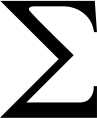
\includegraphics[width=0.225cm]{Bilder/Sigma.png} \nodepart{lower} 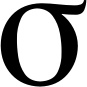
\includegraphics[width=0.225cm]{Bilder/sigma.png}};
        }
        % Draw the left input layer nodes
            \foreach \name / \xn in {1,...,\ni}{
            % This is the same as writing \foreach \name / \y in {1/1,2/2,3/3,4/4}
                \node[neuron,fontscale=15] (Il-\name) at (\xn*\neuronsep-\neuronsep,\y) {$X_{\xn}$};
                \node[above of=Il-\name, node distance=\inout cm] (Inl-\name) {};
                \draw [->,arrows={-Stealth[length=7pt]},densely dotted] (Inl-\name) edge (Il-\name);
            }
            \node[fontscale=15] (Il-dot) at ({(\ni+1)*\neuronsep-\neuronsep},\y) {$\dots$};
            \node[neuron,fontscale=15] (Il-i) at ({(\ni+2)*\neuronsep-\neuronsep},\y) {$X_{i}$};
            \node[above of=Il-i, node distance=\inout cm] (Inl-i) {};
            \draw [->,arrows={-Stealth[length=7pt]},densely dotted] (Inl-i) edge (Il-i);

        % Draw the hidden layer node
            \foreach \name / \xn in {1,...,\nh}{
                \node[neuron] (Hl-\xn) at ({(\ni-1)*\neuronsep/2-\neuronsep/2*(\nh-1)+(\xn-1)*\neuronsep},\y-\layersep) [fontscale=15] {$Z_{\xn}$};
                
                \node[node distance=\inout cm, below of=Hl-\xn] (Hnl) {};
                %\draw [->,arrows={-Stealth[length=7pt]},densely dotted] (Hl-\xn) edge (Hnl);
            }
                \node[fontscale=15] (Hl-dot) at ({(\ni-1)*\neuronsep/2-\neuronsep/2*(\nh+1)+(\nh+1)*\neuronsep},\y-\layersep) {$\dots$};
                \node[neuron,fontscale=15] (Hl-h) at ({(\ni-1)*\neuronsep/2-\neuronsep/2*(\nh+2)+(\nh+2.5)*\neuronsep},\y-\layersep) {$Z_h$};
            
            \foreach \name / \xn in {1,...,\nh,h}{
        % Connect every node in the inner layer with the hidden layer
            \foreach \source in {1,...,\ni,i}
                \draw [->,arrows={-Stealth[length=7pt]}] (Il-\source) edge (Hl-\xn);
                }
                \draw [fill=white,draw=black, dotted] ($(Hl-1)+(\neuronsep/4-.45,\layersep*.625)$) rectangle ($(Hl-h)+(\neuronsep/100,\layersep*.4)$);
                \node[fill=white,inner sep=1pt,fontscale=10] at ($(Hl-1)+({(\nh+1)*\neuronsep/2},\layersep*.5)$) {$\dots\,w_{h,i}\,\dots$};

        % Draw the output layer node
            \foreach \name / \xn in {1,...,\no}{
                \node[neuron,fontscale=15] (Ol-\xn) at ({(\ni-1)*\neuronsep/2-\neuronsep/2*(\no-1)+(\xn-1)*\neuronsep},\y-2*\layersep) {$Y_{\xn}$};
                \node[node distance=\inout cm, below of=Ol-\xn] (Onl) {};
                \draw [->,arrows={-Stealth[length=7pt]},densely dotted] (Ol-\xn) edge (Onl);
            }
                \node[fontscale=15] (Ol-dot) at ({(\ni-1)*\neuronsep/2-\neuronsep/2*(\no+1)+(\no+1)*\neuronsep},\y-2*\layersep)  {$\dots$};
                \node[neuron,fontscale=15] (Ol-o) at ({(\ni-1)*\neuronsep/2-\neuronsep/2*(\no+2)+(\no+2.5)*\neuronsep},\y-2*\layersep)  {$Y_o$};
                \node[node distance=\inout cm, below of=Ol-o] (Onl) {};
                \draw [->,arrows={-Stealth[length=7pt]},densely dotted] (Ol-o) edge (Onl);
            
            \foreach \name / \xn in {1,...,\no,o}{
        % Connect every node in the hidden layer with the output layer
            \foreach \source in {1,...,\nh,h}
                \draw [->,arrows={-Stealth[length=7pt]}] (Hl-\source) edge (Ol-\xn);
                }
                \draw [fill=white,draw=black, dotted] ($(Ol-1)+(\neuronsep/3-1.5,\layersep*.625)$) rectangle ($(Ol-o)+(\neuronsep/2,\layersep*.4)$);
                \node[fill=white,inner sep=1pt,fontscale=10] at ($(Ol-1)+({(\no+1)*\neuronsep/2},\layersep*.5)$) {$\dots\,w_{o,h}\,\dots$};
                
        % Annotate the layers
            \ifthenelse{\ni>\nh}{
                \node[annot,right of=Il-i, node distance=\dlsize cm] (il) {\textbf{Eingabe- schicht}};
                \node[annot,below of=il] (hl) {\textbf{Verdeckte- schicht}};
            }{
                \node[annot,right of=Hl-h, node distance=\dlsize cm] (hl) {\textbf{Verdeckte- schicht}};
                \node[annot,above of=hl] (il) {\textbf{Eingabe- schicht}};
            }
                \node[annot,below of=hl] {\textbf{Ausgabe- schicht}};            
\end{tikzpicture}
    \caption{MLP Das bei der Herleitung des Backpropagation und Levenberg-Marquardt Algorithmuses betrachtet wird.}
    \label{fig:MLP-Algorithm}
\end{figure}


\subsection{Backpropagation}\label{sec:Backpropagation}
%\todo{MLP \citet[90]{dkriesel07}}
Das Backpropagation ist die Kurzform des englischen Begriffes \textit{Backpropagation of error} und zählt zu den Gradientenabstiegsverfahren bei denen die Fehlerverteilung als \glqq hügelige\grqq Landschaft angesehen wird (siehe \autoref{fig:Fehlerlandschaft}). Beim Beginn des Trainings wird die Richtung gesucht in die der Gradient abfällt und ein Schritt in diese Richtung unternommen. Anschließend wiederholt man die Prozedur mehrmals bis es entweder keine Trainingsbeispiele mehr gibt oder der Fehler sich nicht mehr groß verändert und somit ein Fehlerminimum erreicht ist. Das Backpropagation ist eine Erweiterung der Deltaregel und wird analog Hergeleitet. In diesem Abschnitt werden die spezifischen Schritte dargestellt die für das Backpropagation benötigt werden, zur detaillierten Herleitung der Deltaregel wir an dieser Stelle auf den \autoref{sec:deltaregel} verwiesen.
Betrachtet wird nun ein Neuron $Z_h$ in der Mitte des Netzwerkes. Dieses Neuron besitzt eine Menge $H \cdot I$ Verbindungen die zu ihm aber auch eine Menge $O \cdot H$ die von ihm weg führen. Somit übertragen die vorgelagerten Neuronen die gewichtete Information an das Neuron $h$. Formal ergibt sich die Netzeingabe $net_{h}$ des Neurons $h$:
\begin{equation}
net_{h} = \sum_{i \in I} w_{hi} \cdot x_{i} .
\label{gl:neth}
\end{equation}

Nach der Verarbeitung der Eingabeinformationen durch die Aktivierungsfunktion kann die Ausgabe des Neurons $h$ beschrieben werden als:
\begin{equation}
z_{h}= f_{akt}(net_{h}) .
\label{gl:aktiv}
\end{equation}

Wie nun in der Deltaregel zu beobachten war ist die Änderung eines Gewichtes $w_{hi}$ proportional zur negativen Ableitung der Fehlerfunktion nach dem betrachtetem Gewicht. Formal betrachtet ergibt sich
\begin{equation*}
\Delta w_{hi} \propto -  \frac{\partial Err(W_{hi})}{\partial w_{hi}}.
\end{equation*}

Die Änderung der Fehlerfunktion nach dem Gewicht kann auch als Produkt aus der Änderung des Fehlers als Funktion der Änderung der Netzeingabe und der Auswirkung eines Veränderten Gewichtes auf die Netzeingabe betrachtet werden. Dies kann auch geschrieben werden als:
\begin{equation}
\frac{\partial Err(W_{hi})}{\partial w_{hi}} = \frac{\partial Err(W_{hi})}{\partial net_{h}} \cdot \frac{\partial net_{h}}{\partial w_{hi}}.
\label{gl:zerlket2}
\end{equation}

Auch \autoref{gl:vor_xi}, \autoref{gl:xi} und \autoref{gl:neth} kann der zweite Faktor auch geschrieben werden als:
\begin{equation}
\frac{\partial net_{h}}{\partial w_{hi}} = \frac{\partial }{\partial w_{hi}} \sum\limits_{i \in I} w_{hi} x_{i} = x_{i} .
\label{gl:ok_bak}
\end{equation}

Aus der Analogie zwischen der \autoref{gl:zerlket} und \autoref{gl:zerlket2} kann $\delta_{h}$ definiert werden als:
\begin{equation}
\delta_{h}= -\frac{\partial Err(W_{hi})}{\partial net_{h}}  .
\label{gl:deltah_bak}
\end{equation}

Für den Fall das unser betrachtetes Neuron $h$ ein Ausgabeneuron wäre könnte aus der Betrachtung der \autoref{gl:errp} die Fehlerfunktion $Err(W_{hi})$ auch geschrieben werden als
\begin{equation}
Err(W_{hi})= \frac{1}{2} (t_{h}-z_{h})^2 ,
\label{gl:fehler_bak}
\end{equation}
dies wird an dieser Stelle angenommen, um zu verdeutlichen das $Err(W_{hi})$ nur von $z_{h}$ abhängig ist. Es wird nun unterstellt dass $t_h$ unabhängig von $z_h$ ist, was für den Fall eines Ausgabeneurons auch stimmen würde (die Betrachtung des inneren Neurons erfolgt im Anschluss). Unter Berücksichtigung der \autoref{gl:aktiv} kann jetzt $\frac{\partial Err(W_{hi})}{\partial net_{h}}$ mit der Kettenregel umgeformt werden in:
\begin{equation}
\frac{\partial Err(W_{hi})}{\partial net_{h}} = \frac{\partial Err(W_{hi})}{\partial z_{h}} \cdot \frac{\partial z_{h}}{\partial net_{h}}.
\label{gl:ohket_bak}
\end{equation}
Ebenfalls mit Hilfe der \autoref{gl:aktiv} ergibt sich der rechte Faktor zu:
\begin{equation}
\frac{\partial z_{h}}{\partial net_{h}} = f_{akt}'(net_h),
\label{gl:aktiv_neth_bak}
\end{equation}
welches die Ableitung der Aktivierungsfunktion beinhaltet.

Falls $h$ ein Ausgabeneuron wäre, würde aus der Definition für $Err(W_{hi})$ aus \autoref{gl:fehler_bak} folgen:
\begin{equation}
\frac{\partial Err(W_{hi})}{\partial z_{h}} = -(t_h - z_h).
\end{equation}

Befindet sich das zu Betrachtende Neuron aber im inneren des Netzwerkes (wie zu Beginn angenommen) ist $t_h$ abhängig von den nachfolgenden Neuronen. Hieraus Folgt dass $t_h$ eine Funktion von $net_o$ ist und der Fehler $Err(W_{hi})$ ebenfalls von $net_o$ abhängig ist. Somit ergibt sich folgender Formalismus:
\begin{equation*}
Err(W_{hi}) \propto \sum\limits_{o \in O} net_o,
\end{equation*}
wobei $net_o$ gegeben ist durch
\begin{equation}
net_{o} = \sum_{h \in H} w_{oh} \cdot z_{h} .
\label{gl:netl}
\end{equation}

Damit kann $\frac{\partial Err(W_{hi})}{\partial z_{h}}$ mit Hilfer der Kettenregel umgeformt werden in
\begin{equation}
\frac{\partial Err(W_{hi})}{\partial z_{h}} =\sum\limits_{o \in O} \left (  \frac{\partial Err(W_{hi})}{\partial net_{o}} \cdot \frac{\partial net_{o}}{\partial z_{h}} \right ).
\label{gl:sumket_bak}
\end{equation}

Unter Berücksichtigung der \autoref{gl:ok_bak}, \autoref{gl:deltah_bak} und \autoref{gl:netl} folgt, dass die summierten Faktoren der \autoref{gl:sumket_bak} auch geschrieben werden können als:
\begin{equation}
\frac{\partial net_{h}}{\partial z_{h}} = \frac{\partial }{\partial z_{h}} \sum\limits_{h \in H} w_{oh} \cdot z_{h} = w_{oh} .
\label{gl:whl_bak}
\end{equation}
\begin{equation}
\frac{\partial Err(W_{hi})}{\partial net_{o}} = -\delta_o .
\label{gl:deltal_bak}
\end{equation}

Durch das Einsetzen der \autoref{gl:whl_bak} und \autoref{gl:deltal_bak} in \autoref{gl:sumket_bak} ergibt sich:
\begin{equation}
\frac{\partial Err(W_{hi})}{\partial z_{h}} =\sum\limits_{o \in O}  -\delta_o \cdot w_{oh} .
\label{gl:sumketlos_bak}
\end{equation}

Gefolgt vom Einsetzen der \autoref{gl:sumketlos_bak} und \autoref{gl:aktiv_neth_bak} in \autoref{gl:ohket_bak} und \autoref{gl:deltah_bak} folgt:
\begin{equation}
\delta_{h}= -\frac{\partial Err(W_{hi})}{\partial net_{h}} = f_{akt}'(net_h) \cdot \sum\limits_{o \in O}  \delta_o \cdot w_{oh}.
\label{gl:deltahinnen_bak}
\end{equation}

Aus \autoref{gl:deltahinnen_bak}, \autoref{gl:ok_bak} und \autoref{gl:fertig_delta} kann schließlich die Änderung des Gewichtes $w_{hi}$ eines innerhalb des Netzwerkes liegenden Neurons $h$ bestimmt werden durch
\begin{equation}
\Delta w_{hi} = \alpha \cdot x_{i} \cdot f_{akt}'(net_h) \cdot \sum\limits_{o \in O}  \delta_o \cdot w_{oh}  .
\label{gl:fertiginnen_bak}
\end{equation}

Allgemein betrachtet kann, unter Berücksichtigung der Deltaregel für das Onlinelernverfahren (\autoref{gl:fertig_delta}), das Backpropagation-Verfahren zusammengefasst werden in\,\citef[89 ff]{dkriesel07}
\begin{align}
\nonumber & \Delta w_{hi}  = \alpha \cdot x_{i} \cdot \delta_h, \quad \text{mit}\\
&\delta_h = \left \{
\begin{aligned}
&f_{akt}'(net_h) \cdot (t_h - z_h) &[\text{ wenn }  h \text{ ein au\ss enliegendes Neuron ist }]\\ 
&f_{akt}'(net_h) \cdot \sum\limits_{o \in O}  \delta_o \cdot w_{oh} &[\text{ wenn }  h \text{ ein innenliegendes Neuron ist }]\\
\end{aligned}
.
\right.
\label{gl:fertigbeide_bak}
\end{align}

\textbf{Algorithmus:}\,\citef[289]{Fausett1993}

Das  Backpropagation-Verfahrens besteht aus drei Schritten. Zunächst werden die Information von der Eingabe zur Ausgabeschicht und somit nach "vorne" (engl.: forward) durchgegeben. Als nächstes wird die Abweichung (auch als Fehler bezeichnet) zwischen dem errechneten und gewünschten Wert bestimmt. Die Abweichung wird anschließend von der Ausgebe hin zur Eingabeschicht "zurück" (engl.: back) gereicht und dazu genutzt die Gewichte der einzelnen Schichten anzupassen.

\begin{itemize}
\item[\textbf{$\bullet$}] Schritt 1: Initialisiere die Gewichte zu kleinen zufälligen Werten.
\item[\textbf{$\bullet$}] Schritt 2: Solange die Abbruchbedingung falsch ist widerhole Schritt 3--10.
\item[\textbf{$\bullet$}] Schritt 3: Wiederhole für jedes Trainingspaar Schritt 4--9.
\end{itemize}

\textbf{\textit{Feedforward:}}
\begin{itemize}
\item[\textbf{$\bullet$}] Schritt 4: Jedes Eingabeneuron $(X_{i}, i=1,\dots,I)$ bekommt das Eingabesignal $x_{i}$ und leitet es zu jedem Neuron der nachfolgenden Schicht (verdeckte Schicht).

\item[\textbf{$\bullet$}] Schritt 5: Jedes der verdeckten Neuronen $(Z_{h}, h=1,\dots,H)$ summiert das gewichtete Eingabesignal
\begin{equation}
net_{h}=\sum\limits_{i \in I} x_{i}w_{hi},
\end{equation}
wendet auf das Ergebnis die Aktivierungsfunktion an 
\begin{equation}
z_{h}=f_{akt}(net_{h})
\end{equation}
und leitet das Resultat an jedes Neuron der nachfolgenden Schicht (Ausgabeschicht).

\item[\textbf{$\bullet$}] Schritt 6: Jedes der Ausgabeneuronen $(Y_{o}, o=1,\dots,O)$ summiert das gewichtete Eingabesignal 
\begin{equation}
net_{o}=\sum\limits_{h \in H} z_{h}w_{oh},
\end{equation}
wendet auf das Ergebnis die Aktivierungsfunktion an 
\begin{equation}
y_{o}=f_{akt}(net_{o}).
\end{equation}
\end{itemize}

\textbf{\textit{Backpropagation:}}
\begin{itemize}
\item[\textbf{$\bullet$}] Schritt 7: Jedes Ausgabeneuron $(Y_{o}, o=1,\dots,O)$ bekommt die zum Eingabesignal passende Lösung $t_{o}$ und berechnet den Fehleranpassungsterm 
\begin{equation}
\delta_{o}=(t_{o}-y_{o})f_{akt}'(net_{o}),
\end{equation}
kalkuliert anschließend die Gewichtsänderung 
\begin{equation}
\Delta w_{oh}=\alpha \delta_{o} z_{h}
\end{equation}
und leitet den Fehleranpassungsterm $\delta_{o}$ an die unterliegende Schicht.

\item[\textbf{$\bullet$}] Schritt 8: Jedes verdeckte Neuron $(Z_{h}, h=1,\dots,H)$ bekommt die Summe aus Fehleranpassungsthermen $\delta_o$ und Gewichten $w_{oh}$ von der vorgelagerten Schicht und multipliziert die Summe mit der abgeleiteten Aktivierungsfunktion, um seinen Fehleranpassungstherm 
\begin{equation}
\delta_{h}=f_{akt}'(net_{h}) \cdot \sum\limits_{o \in O} \delta_{o} \cdot w_{oh}
\end{equation}
zu bestimmen. Der Fehleranpassungsterm wird anschließend benutzt, um die Gewichtsanpassung 
\begin{equation}
\Delta w_{hi}=\alpha \delta_{h} x_{i}
\end{equation}
zu berechnen.
\end{itemize}

\textbf{\textit{Anpassen der Gewichte:}}
\begin{itemize}
\item[\textbf{$\bullet$}] Schritt 9: Jedes Ausgabeneuron $(Y_{o}, o=1,\dots,O)$ passt seine Gewichte an: 
\begin{equation}
w_{oh}(\text{neu})=w_{oh}(\text{alt})+\Delta w_{oh}.
\end{equation}
Jedes verdeckte Neuron $(Z_{h}, h=1,\dots,H)$ passt seine Gewichte an:
\begin{equation}
w_{hi}(\text{neu})=w_{hi}(\text{alt})+\Delta w_{hi}.
\end{equation}

\item[\textbf{$\bullet$}] Schritt 9: Überprüfe die Abbruchbedingung.
\end{itemize}

\subsection{Levenberg-Marquardt}\label{sec:LM_herleitung}



%\subsubsection{Levenberg-Marquardt}
Der Levenberg-Marquardt (LM)-Algorithmus baut auf dem klassischen Gradientenabstiegsverfahren auf, welches auch als Backpropagation bezeichnet und in \autoref{sec:Backpropagation} hergeleitet wird. Es wird an dieser Stelle nun auch von der Fehlerfunktion $Err_{po}(W)$ über alle Trainingsbeispiele $P$ in der folgenden Form Ausgegangen:

\begin{equation}
Err_{po}(W)= \frac{1}{2} \sum\limits_{p \in P} \sum\limits_{o \in O} e_{po}^2,
\label{gl:LM_fehler}
\end{equation}
mit
\begin{equation}
e_{po}=(t_{po}-y_{po}).
\end{equation}

Das Gradientenabstiegsverfahren beruht auf der ersten Ableitung der Fehlerfunktion und kann wie folgt als Gradientenvektor dargestellt werden:
\begin{equation}
\nabla Err_{po}(W)= \frac{\partial Err_{po}(W)}{\partial w_{on}}= \left [ \frac{Err_{1p}(W)}{\partial w_{11}} , \frac{Err_{1p}(W)}{\partial w_{12}}, \dots,  \frac{\partial Err_{po}(W)}{\partial w_{on}}  \right ]^T,
\label{gl:LM_bp_err}
\end{equation}
mit $n \in N$ und $N= I \cdot H + H \cdot O$ als Menge aller Gewichte eines Netzwerks.

Der Trainingsprozess des Algorythmuses konvergiert asymptotisch und nah an einem Minimum werden die Komponenten des Gradientenvektors sehr klein und somit die Gewichtsänderung sehr gering. Der Übersichtshalber wird die Ableitung der Fehlerfunktion umbenannt in einen Gradienten $g$ mit:
\begin{equation}
g= \nabla Err_{po}(W).
\label{gl:LM_gradient}
\end{equation}

Mit der \autoref{gl:LM_gradient} kann die Gewichtsänderung des Gradientenabstiegverfahrens ausgedrückt werden als:
\begin{equation}
\Delta w= - \alpha g,
\label{gl:LM_bp_delta-w}
\end{equation}
wobei $\alpha$ die Schrittweite bzw. die Lernrate repräsentiert.

Bei der Newtonmethode wird nun angenommen, dass die Gradienten $g_{po}$ aller Trainingsbeispiele $P$ des Ausgabeneurons $o$ in einer nichtlinearen Beziehung $F_{po}$ zwischen den Gewichten $w_{oh}$ und den jeweiligen Komponenten der Gradienten stehen. Formel kann dies ausgedrückt werden in
\begin{align}
\left \{
\begin{aligned}
&g_{p1}= F_{p1}(w_{11},w_{12},\dots, w_{1n})\\ 
&g_{p2}= F_{p2}(w_{21},w_{22},\dots, w_{2n})\\
&\dots\\
&g_{po}= F_{po}(w_{o1},w_{o2},\dots, w_{on})\\
\end{aligned}
.
\right.
\label{gl:LM_g1}
\end{align}

Mit der Taylor-Näherung erster Ordnung kann die nichtlineare Beziehung $F$ und somit auch der Gradient $g$ ausgedrückt werden als:
\begin{equation}
g_{po} \approx g_{po}(w_{o0}) + \sum\limits_{n \in N} \frac{\partial g_{po}}{\partial w_{on}} \Delta w_{on}.
\label{gl:LM_g2}
\end{equation}

Durch das Einsetzen der \autoref{gl:LM_bp} und \autoref{gl:LM_gradient} kann geschlussfolgert werden, dass
\begin{equation}
\frac{\partial g_{po}}{\partial w_{on}} = \frac{\partial \left ( \frac{\partial Err_{po}(W)}{\partial w_{on}} \right )}{\partial w_{on}} = \frac{\partial^2  Err_{po}(W)}{\partial w_{on} \partial w_{on}}.
\label{gl:LM_g3}
\end{equation}

Nun wird \autoref{gl:LM_g3} in \autoref{gl:LM_g2} eingesetzt und der Gradientenvektor $g_{po}$ kann geschrieben werden als:
\begin{equation}
g_{po} \approx g_{po}(w_{o0}) + \sum\limits_{n \in N} \frac{\partial^2 Err_{po}(W)}{\partial w_{on} \partial w_{on}} \Delta w_{on} .
\label{gl:LM_g4}
\end{equation}

Um nun ein Minimum der Fehlerfunktion zu finden müssen die Gradienten Nullgesetzt werden. Somit wird aus \autoref{gl:LM_g4}
\begin{equation}
0 \approx g_{po}(w_{o0}) + \sum\limits_{n \in N} \frac{\partial^2 Err_{po}(W)}{\partial w_{on} \partial w_{on}} \Delta w_{on} .
\label{gl:LM_g5}
\end{equation}

Durch das Einsetzen der \autoref{gl:LM_bp} und \autoref{gl:LM_gradient} in \autoref{gl:LM_g5} ergibt sich
\begin{equation}
-\frac{\partial Err_{po}(W)}{\partial w_{o}}  = -g_{po}(w_{o0}) \approx \sum\limits_{n \in N} \frac{\partial^2 Err_{po}(W)}{\partial w_{on} \partial w_{on}} \Delta w_{on} .
\label{gl:LM_g6}
\end{equation}

Hieraus ergeben sich $P \text{mal} O$ Gleichungen. Durch das Lösen dieser Gleichungen kann $\Delta w_{on}$ bestimmt werden. Die \autoref{gl:LM_g6} kann auch in Matrizen-Form geschrieben werden

\begin{equation}
 \begin{bmatrix}
  -g_{p1}   \\
  -g_{p2}   \\
  \vdots    \\
  -g_{po}   \\ 
 \end{bmatrix}
 =
  \begin{bmatrix}
  -\frac{\partial Err_{p1}(W)}{\partial w_{1}}   \\
  -\frac{\partial Err_{p2}(W)}{\partial w_{2}}   \\
  \vdots    \\
  -\frac{\partial Err_{po}(W)}{\partial w_{o}}   \\ 
 \end{bmatrix}
 =
 \begin{bmatrix}
    \frac{\partial^2 Err_{p1}}{\partial w_{1n} \partial w_{o1}} & \frac{\partial^2 Err_{p1}}{\partial w_{1n} \partial w_{o2}}  & \dots  & \frac{\partial^2 Err_{p1}(W)}{\partial w_{on} \partial w_{on}} \\
    \frac{\partial^2 Err_{p2}}{\partial w_{2n} \partial w_{o1}} & \frac{\partial^2 Err_{p2}}{\partial w_{2n} \partial w_{o2}}  & \dots  & \frac{\partial^2 Err_{p2}(W)}{\partial w_{on} \partial w_{on}} \\
    \vdots & \vdots & \ddots & \vdots \\
    \frac{\partial^2 Err_{po}}{\partial w_{on} \partial w_{o1}} & \frac{\partial^2 Err_{po}}{\partial w_{on} \partial w_{o2}}  & \dots  & \frac{\partial^2 Err_{po}(W)}{\partial w_{on} \partial w_{on}} \\
 \end{bmatrix}
\times
 \begin{bmatrix}
  \Delta w_{1n}  \\
  \Delta w_{2n}  \\
  \vdots    \\
  \Delta w_{on}   \\ 
 \end{bmatrix}
\label{gl:LM_matrix-schreibweise}
\end{equation}

Die Ableitungen zweiter Ordnung enthaltene Matrix wird auch als Hesse-Matrix $H$ bezeichnet
\begin{equation}
H
 =
 \begin{bmatrix}
    \frac{\partial^2 Err_{p1}}{\partial w_{1n} \partial w_{o1}} & \frac{\partial^2 Err_{p1}}{\partial w_{1n} \partial w_{o2}}  & \dots  & \frac{\partial^2 Err_{p1}(W)}{\partial w_{on} \partial w_{on}} \\
    \frac{\partial^2 Err_{p2}}{\partial w_{2n} \partial w_{o1}} & \frac{\partial^2 Err_{p2}}{\partial w_{2n} \partial w_{o2}}  & \dots  & \frac{\partial^2 Err_{p2}(W)}{\partial w_{on} \partial w_{on}} \\
    \vdots & \vdots & \ddots & \vdots \\
    \frac{\partial^2 Err_{po}}{\partial w_{on} \partial w_{o1}} & \frac{\partial^2 Err_{po}}{\partial w_{on} \partial w_{o2}}  & \dots  & \frac{\partial^2 Err_{po}(W)}{\partial w_{on} \partial w_{on}} \\
 \label{gl:LM_hesse-mat}
 \end{bmatrix}
 .
\end{equation}

Die \autoref{gl:LM_matrix-schreibweise} kann in Kurzform dargestellt werden als:
\begin{equation}
-g=H \cdot \Delta w
\end{equation}

und die Umstellung nach $\Delta w$ ergibt
\begin{equation}
\Delta w =-H^{-1} \cdot g.
\label{gl:LM_hesse}
\end{equation}

Beim Vergleich der \autoref{gl:LM_bp_delta-w} und \autoref{gl:LM_hesse} wird ersichtlich, dass die Hesse-Matrix beim Gradientenabstieg die passenden Schrittweiten liefert.

Wenn man die Newtonmethode zur Gewichtsanpassung verwenden möchte, so müssen die Ableitungen zweiter Ordnung berechnet werden, um die Hesse-Matrix zu erhalten. dies erweist sich in einigen fällen als nicht trivial. Um diesen Prozess zu vereinfachen wird beim Gauss-Newton-Algorithmus die Jacobi-Matrix $J$ eingeführt
\begin{equation}
J
=
 \begin{bmatrix}
    \frac{\partial e_{11}}{\partial w_{11}} & \frac{\partial e_{11}}{\partial w_{12}}  & \dots  & \frac{\partial e_{11}}{\partial w_{on}} \\
    \frac{\partial e_{12}}{\partial w_{21}} & \frac{\partial e_{12}}{\partial w_{22}}  & \dots  & \frac{\partial e_{12}}{\partial w_{on}} \\
    \vdots & \vdots & \ddots & \vdots \\
    \frac{\partial e_{1o}}{\partial w_{o1}} & \frac{\partial e_{1o}}{\partial w_{o2}}  & \dots  & \frac{\partial e_{1o}}{\partial w_{on}} \\
    \frac{\partial e_{2o}}{\partial w_{o1}} & \frac{\partial e_{2o}}{\partial w_{o2}}  & \dots  & \frac{\partial e_{2o}}{\partial w_{on}} \\
    \vdots & \vdots & \ddots & \vdots \\
    \frac{\partial e_{po}}{\partial w_{o1}} & \frac{\partial e_{po}}{\partial w_{o2}}  & \dots  & \frac{\partial e_{po}}{\partial w_{on}} \\
 \end{bmatrix}
,
\end{equation}
wobei

\begin{align}
 \frac{\partial e_{p \alpha}}{\partial w_{\beta n}}
\left \{
\begin{aligned}
& \frac{\partial e_{p o}}{\partial w_{o n}} \quad \text{wenn} \quad \alpha=\beta \quad \alpha,\beta=1,\dots,o, \\
& 0 \quad \qquad \text{sonst}.
\end{aligned}
\right.
\label{gl:LM_fuellen}
\end{align}


Nach dem Einsetzen der \autoref{gl:LM_fehler} in \autoref{gl:LM_bp_err} und \autoref{gl:LM_gradient} können die einzelnen Elemente des Gradientenvektors berechnet werden als:
\begin{equation}
g_{po} = \frac{\partial Err_{po}(W)}{\partial w_{on}} = \frac{\partial \left (\frac{1}{2} \sum_{p \in P} \sum_{o \in O} e_{po}^2 \right )}{\partial w_{on}} 
=
\sum_{p \in P} \sum_{o \in O} \left ( \frac{\partial e_{po}}{\partial w_{on}} e_{po} \right )
\label{gl:LM_g-J}
\end{equation}

Verkürzt kann der Zusammenhang zwischen der Jacobi-Matrix und dem Gradientenvektor geschrieben werden als:
\begin{equation}
g = Je,
\label{gl:LM_Je}
\end{equation}
wobei der Fehlervektor folgende Form aufweist
\begin{equation}
e= \left [ e_{11}, e_{12}, \dots, e_{1o}, \dots, e_{p1}, e_{p2}, \dots, e_{po} \right ]^T.
\label{gl:LM_bp}
\end{equation}

Nach dem Einsetzen der \autoref{gl:LM_fehler} in \autoref{gl:LM_hesse-mat} können die Elemente der Hesse-Matrix berechnet werden durch
\begin{equation}
h_{po} = \frac{\partial^2 Err_{po}(W)}{\partial w_{on} \partial w_{on}} = \frac{\partial \left (\frac{1}{2} \sum_{p \in P} \sum_{o \in O} e_{po}^2 \right )}{\partial w_{on} \partial w_{on}} 
=
\sum_{p \in P} \sum_{o \in O} \frac{\partial e_{po}}{\partial w_{on}} \frac{\partial e_{po}}{\partial w_{on}} + S_{on}.
\label{gl:LM-h}
\end{equation}

Dabei setzt sich $S_{on}$ zusammen aus:
\begin{equation}
S_{on} = \sum_{p \in P} \sum_{o \in O} \frac{\partial^2 e_{po}}{\partial w_{on} \partial w_{on}} e_{po}.
\label{gl:LM_S}
\end{equation}

Bei der Newtonmethode wird nun angenommen, dass $S_{on}$ annähernd Null ist\,\citef[990]{Hagan1994} und somit kann die Hesse-Matrix ausgedrückt werden als:
\begin{equation}
H = J^T J.
\label{gl:LM_JJ}
\end{equation}

Durch die Kombination der \autoref{gl:LM_hesse}, \autoref{gl:LM_Je} und \autoref{gl:LM_JJ} kann die Gewichtsänderung des Gauss-Newton-Algorithmus beschrieben werden als:
\begin{equation}
\Delta w =-(J^T J)^{-1} J e.
\label{gl:LM_GNA}
\end{equation}

Der Vorteil des Gauss-Newton-Algorithmuses gegenüber dem Newtonmethode besteht darin, dass anstatt der zweifachen Ableitung der Fehlerfunktion durch die Jacobi-Matix nur noch die einfache Ableitung benötigt wird. Einen Nachteil den aber beide Ansätze gemeinsam haben ist, dass die Hesse-Matrix bzw. die $J^T J$-Matrix in einigen Fällen nicht invertierbar sind. Um sicher zu gehen dass die angenäherte Hesse-Matrix invertierbar ist, wird im Levenberg-Marquardt-Algorithmus ein zusätzlicher Term eingeführt:
\begin{equation}
H \approx J^T J + \mu I.
\label{gl:LM_lm-H}
\end{equation}

Hierbei ist $\mu$ stets positiv und wird als Kombinationskoeffizient bezeichnet. I ist die Einheitsmatrix.

Durch den zusätzlichen Term in \autoref{gl:LM_lm-H} wird die Hauptdiagonale der Hesse-Matrix größer als Null sein und damit ist sichergestellt, dass $H$ immer invertierbar ist. Mit \autoref{gl:LM_GNA} und \autoref{gl:LM_lm-H} kann der Levenberg-Marquard-Algorithmus ausgedrückt werden als:
\begin{equation}
\Delta w =-(J^T J + \mu I)^{-1} J e.
\label{gl:LM_lm-delta-w}
\end{equation}

Der Levenberg-Marquard-Algorithmus kann als Kombination zwischen dem klassischen Gradientenabstiegsverfahren und dem Gauss-Newton-Algorithmus angesehen werden. Wenn der Kombinationskoeffizient $\mu$ sich sehr nah an der Null befindet so nährt sich die \autoref{gl:LM_lm-delta-w} der \autoref{gl:LM_GNA} an und damit dem Gauss-Newton-Algorithmus. Ist der Kombinationskoeffizient aber sehr groß so nähert sich die \autoref{gl:LM_lm-delta-w} der \autoref{gl:LM_bp_delta-w} an und so bekommt das klassische Gradientenabstiegsverfahren die größere Gewichtung. Für den Fall, dass $\mu$ sehr Groß wird kann es als Lernrate mit folgender Beziehung angesehen werden:\,\citef[12-1 ff]{Wilamowski2011}
\begin{equation}
\alpha = \frac{1}{\mu}.
\label{gl:LM_lernrate}
\end{equation}

Der klassische LM-Albgorithmus ist eine Offline-Lernmethode in der die Jacobi-Matrix alle Gewichte eines Netzwerks enthält und somit die Gewichtsänderung aller Gewichte in einem Schritt berechnet. Dies hat zur Folge, dass mit steigender Anzahl der Neuronen eines Netzwerks die Anzahl der Gewichte dieses Netzwerks ebenfalls steigt. Dies resultiert in einer größeren Jacobimatrix, was zu einem hohen Speicher- und Berechnungsaufwand führen kann. Um den Speicherbedarf gering zu halten wurde in dieser Arbeit der \textit{Layer-by-Layer} LM-Algorithmus von \citet{Kwak2012} in abgewandelter Form implementiert. Hier wird eine eigene Jacobi-Matrix für jede Gewichtsschicht erstellt und dementsprechend auch die Gewichtsänderung für die jeweilige Schicht einzeln berechnet. Durch die geringere Anzahl an Gewichten werden die einzelnen Jacobi-Matrizen kleiner und somit sinkt auch der Specherbedarf pro Matrix.\\

\textbf{Algorithmus:}\,\citef{Kwak2012}\\
Im Allgemeinen besteht der LM-Algorithmus aus den gleichen drei Schritten wie das Backpropagation Verfahren. Zunächst werden die Informationen der Eingabeschicht zur Ausgabeschicht durchgereicht. Im nächsten Schritt werden die Abweichungen zwischen errechneten Werten und der erwarteten Lösung berechnet. Anschließend werden die Änderungen genutzt, um die Gewichte der einzelnen Schichten anzupassen. Der Unterschied liegt in der Art wie die Abweichungen genutzt werden, um die Gewichtsänderung zu bestimmen.

\begin{itemize}
\item[\textbf{$\bullet$}] Schritt 1: Initialisiere die Gewichte zu kleinen zufälligen Werten und lege die Kombinationskoeffizienten $\mu_o$, $\mu_h$ und den Abklingfaktor $\lambda$ sowie die maximale Anzahl an Iterationen und den vertretbaren Durchschnittsfehler $Err$ fest.

\item[\textbf{$\bullet$}] Schritt 2: Solange die maximale Anzahl an Iterationen nicht überschritten ist oder der Durchschnittsfehler
\begin{equation}
Err= \frac{1}{p} \sum\limits_{p \in P} \sum\limits_{o \in O} e_{po}^2, \quad e_{po}=(t_{po}-y_{po})
\label{gl:alg_LM_err}
\end{equation}
nicht unter den gewünschten Wert fällt wiederhole Schritt 3--14.

\item[\textbf{$\bullet$}] Schritt 3: Jedes Eingabeneuron $(X_{i}, i=1,\dots,I)$ bekommt das Eingabesignal $x_{i}$ und leitet es zu jedem Neuron der nachfolgenden Schicht (verdeckte Schicht).

\item[\textbf{$\bullet$}] Schritt 4: Jedes der verdeckten Neuronen $(Z_{h}, h=1,\dots,H)$ summiert das gewichtete Eingabesignal
\begin{equation}
net_{h}=\sum\limits_{i \in I} x_{i}w_{hi},
\end{equation}
wendet auf das Ergebnis die Aktivierungsfunktion an 
\begin{equation}
z_{h}=f_{act}(net_{h})
\end{equation}
und leitet das Resultat an jedes Neuron der nachfolgenden Schicht (Ausgabeschicht).

\item[\textbf{$\bullet$}] Schritt 5: Jedes der Ausgabeneuronen $(Y_{o}, o=1,\dots,O)$ summiert das gewichtete Eingabesignal 
\begin{equation}
net_{o}=\sum\limits_{h \in H} z_{h}w_{oh}
\end{equation}
und wendet auf das Ergebnis die Aktivierungsfunktion an 
\begin{equation}
y_{o}=f_{act}(net_{o}).
\end{equation}

\item[\textbf{$\bullet$}] Schritt 6: Wiederhole Schritt 3 -- 5 für alle Trainingsbeispiele p und Bestimme mit \autoref{gl:alg_LM_err} den Durchschnittsfehler $Err$.

\item[\textbf{$\bullet$}] Schritt 7: Bestimme die Jacobi-Matrix $J_{o}$ mit\,\footnote{Wird ein Index ohne die Trainingsbeispiellaufvariable p angegeben bedeutet dies, dass die Matrix bzw. der Vektor die gesamten Trainingsbeispiele P enthält. Ausgenommen hiervon sind die skalaren größen der Kombinationskoeffizienten $\mu_o$ und $\mu_h$.}
\begin{equation}
J_{o}= \left \{ j_{po} \right \}, j_{po}=-f_{act}'(net_{po}) \cdot y_{po}.
\end{equation}

\item[\textbf{$\bullet$}] Schritt 8: Benutze die Jacobi-Matrix $J_{o}$, um die Gewichtsanpassung
%\begin{equation}
%\begin{align}
\begin{equation}
\Delta w_{oh}=-(J_{o}^T J_{o} + \mu_{o} J_{o})^{-1} J_{o} e_{o}\\
\end{equation}
mit
\begin{equation}
e_{o}= \left [ e_{11}, e_{12}, \dots, e_{1o}, \dots, e_{p1}, e_{p2}, \dots, e_{po} \right ]^T\\
\end{equation}
zu berechnen.

\item[\textbf{$\bullet$}] Schritt 9: Berechne den temporären Durchschnittsfehler $Err(\text{temp})$ mit Hilfe von
\begin{equation}
w_{oh}(\text{temp})= w_{oh} + \Delta w_{oh},
\end{equation}
wobei die Schritte 3--6 wiederholt werden.\\
Zudem wird verglichen:\\
Wenn $Err(\text{temp}) > Err$ dann
\begin{align*}
&\mu_o = \mu_o / \lambda, \\
&\text{gehe zu Schritt 8.}
\end{align*}
Sonst
\begin{align*}
&\mu_o = \mu_o \cdot \lambda, \\
&Err=Err(\text{temp}), w_{oh}=w_{oh}(\text{temp}).
\end{align*}

\item[\textbf{$\bullet$}] Schritt 10: Nun wird für jedes verdeckte Neuron $(Z_h,h=1,\dots,H)$ der rückgeführte Fehler $e_{h}$ für alle Trainingsbeispiele berechnet:
\begin{equation}
e_{h}= \left [ e_{11}, e_{12}, \dots, e_{1h}, \dots, e_{p1}, e_{p2}, \dots, e_{ph} \right ]^T\\
\end{equation}
mit
\begin{equation}
e_{ph} = \left (    \sum\limits_{o \in O} w_{oh} f_{act}'(net_{o}) (t_{po}-y_{po})  \right )  - y_{ph}.
\end{equation}


\item[\textbf{$\bullet$}] Schritt 11: Bestimme nun die Jacobi-Matrix $J_{h}$ der verdeckten Schicht mit
\begin{equation}
J_{h}= \left \{ j_{ph} \right \}, j_{ph}=-f_{act}'(net_{ph}) \cdot z_{ph}.
\end{equation}

\item[\textbf{$\bullet$}] Schritt 12: Benutze die Jacobi-Matrix $J_{h}$, um die Gewichtsanpassung 
\begin{equation}
\Delta w_{hi}=-(J_{h}^T J_{h} + \mu_{h} J_{h})^{-1} J_{h} e_{h}.
\end{equation}
zu berechnen.

\item[\textbf{$\bullet$}] Schritt 13: Berechne nun ebenfalls für die verdeckte Schicht den temporären Durchschnittsfehler $Err(\text{temp})$ mit Hilfe von
\begin{equation}
w_{hi}(\text{temp})= w_{hi} + \Delta w_{hi},
\end{equation}
wobei die Schritte 3--6 wiederholt werden.\\
Zudem wird verglichen:\\
Wenn $Err(\text{temp}) > Err$ dann
\begin{align*}
&\mu_h = \mu_h / \lambda, \\
&\text{gehe zu Schritt 12.}
\end{align*}
Sonst
\begin{align*}
&\mu_h = \mu_h \cdot \lambda, \\
&Err=Err(\text{temp}), w_{hi}=w_{hi}(\text{temp}).
\end{align*}

\item[\textbf{$\bullet$}] Schritt 14: Gehe zu Schritt 2.
\end{itemize}

\subsection{Vergleich der Lernalgorithmen}\label{sec:vergleich_la}

Bei der Betrachtung beider Lernalgorithmen ist das standard Backpropagation-Verfahren simpler aufgebaut als der LM-Algorithmus. Das BP benötigt weder die Hesse- noch die Jacobi-Matrix und lässt sich somit einfacher implementieren. Andererseits muss die Schrittweite $\alpha$ iterativ für jeden Einsatzzweck neu bestimmt werden. Zusätzlich muss auch die optimale Anzahl der Epochen\,\footnote{Als Epoche wird ein Trainingsdurchlauf mit den gesamten Trainingsdaten bezeichnet. Die Anzahl der Epochen gibt also an wie oft das Netzwerk mit den selben Daten trainiert wurde.%
%Bei mehreren Epochen wird das Netzwerk also mehrmals mit den gleichen Daten trainiert.
} iterativ bestimmt werden. Da es zur bestimmung dieser keine Patentrezepte gibt. Je höher die Anzahl der Epochen ist desto besser Lernt das Netzwerk die Trainingsdaten, braucht aber gleichzeitig länger für das Training. Bei einer zu hohen Anzahl an verdeckten Neuronen oder Epochen kann das Netzwerk die Trainingsdaten auch \glqq Auswendiglernen\grqq~dies bedeutet, dass das Netzwerk zwar die Trainingsdaten gut wiedergeben kann aber schlecht generalisiert und bei zuvor \glqq ungesehenen\grqq~Daten zu fehlerhaften Ergebnissen führt. In der Literatur wird hierfür empfohlen den Datensatz in ein Trainings- und Testset zu unterteilen. Wobei das Testset zur Evaluierung des Netzwerkes dient.\,\citef[58 ff]{dkriesel07}

Der Levenberg-Marquardt Algorithmus weist einen komplexeren Algorithmus auf. So müssen zu Beginn zwar die Anfangswerte für die Kombinationskoeffizienten manuell gesetzt werden, die optimalen Werte aber werden während des Trainings autonom gesetzt. Zusätzlich muss der vertretbare Durchschnittsfehler und die maximale Anzahl an Iterationen zu Beginn festgelegt werden. Hier ist zu beachten, dass das Netzwerk so oft versuchen wird den angegebenen Fehler zu unterschreiten bis die Anzahl an Iterationen erreicht ist. Da der Algorithmus bei jeder Schicht die Kombinationskoeffizienten solange verändert bis ein kleinerer Fehler erreicht wird kann das Netzwerk bei zu klein eingestellten vertretbaren Fehler und hoher Anzahl an Iterationen sehr lange für das Training benötigen. Zusätzlich ist es möglich dass der Algorithmus in der dargestellten Form trotz Veränderung der Kombinationskoeffizienten keinen geringeren Fehler Wert erreicht und so in eine Endlosschleife gerät. Bei der Implementierung des Algorithmus wurde daher eine Zählervariable hinzugefügt die den Versuch einen geringeren Fehler zu erreichen nach dem 10. Mal abbricht. Unterschreitet das Netzwerk beim Training den vordefinierten Fehlerwert bevor die Iterationen ihren Maximalwert erreichen so wird das Training ebenfalls beendet und so ein \glqq Auswendiglernen\grqq~vermieden. In der Literatur wird dem LM-Algorithmus zusätzlich eine schnellere Konvergenz zugesprochen.\,\citef[12-7]{Wilamowski2011} Dies ist vergleichbar mit einem schnelleren Lernprozess. Da die Jacobi-Matrix in dem klassischen LM-Algorithmus zu hohem Speicherbedarf führen kann, ist dieser Algorithmus aber auf Leistungsfähige Computer angewiesen. 

Im Hinblick auf die Vorhersagegenauigkeit sind beide Algorithmen von den spezifischen Eigenschaften des MLP abhängig. In beiden Algorithmen werden die Gewichte zu Beginn des Trainings zufällig initialisiert. Somit startet jedes Training an einem anderen Ort in der Fehlerlandschaft (siehe \autoref{fig:Fehlerlandschaft}) und kann in unterschiedlichen lokalen Minima münden. Dies bedeutet, dass Netzwerke mit gleichem Aufbau und gleicher Anzahl an Neuronen in jeder Schicht aber mit unterschiedlichen Anfangsgewichten nach dem Training mit den selben Daten zu unterschiedlichen Ergebnissen führen können. In der Literatur wird bei der Bestimmung der optimalen Netzparameter ein Netzwerk mit gleichen Parametern mehrmals initialisiert, trainiert und die Ergebnisse gemittelt, um die Einflüsse von \glqq schlechten\grqq~Minima zu reduzieren. Einen Konsens über die zum Mittelwert beitragenden Neuinitialisierungen gebt es aber nicht. So führen \citet{Domanski2017} fünf, \citet{Keles2016} sechs und \citet{Monteiro2016} 20 Neuinitialisierungen durch. Eine höhere Anzahl führt hier zu einem geringeren Einfluss der \glqq schlechten\grqq~Minima erhöht aber gleichzeitig die Berechnungsdauer.

Desweiteren ist die Anzahl der Eingabeneuronen durch die Anzahl an Eingabevariablen und die Anzahl der Ausgabeneuronen durch die zu bestimmenden Größen bedingt. Die optimale Anzahl an verdeckten Neuronen muss aber in beiden Algorithmen bei jeder Aufgabe neu bestimmt werden. Des weiteren übt die Aktivierungsfunktion einen Einfluss auf die Vorhersagegenauigkeit aus. Während lineare Aktivierungsfunktionen in der Lage sind lineare Zusammenhänge in Daten zu erkennen so bedarf es nichtlinearer Aktivierungsfunktionen, um nichtlineare Zusammenhänge abbilden zu können.\,\citef[194]{dkriesel07} Zusätzlich wird bei der Implementierung der Algorithmen oft ein sogenanntes Bias-Neuron zur Eingabe- und jeder verdeckten Schicht hinzugefügt. Das Bias-Neuron verfügt ebenfalls über eine gewichtete Verbindung zur nachfolgenden Schicht, gibt aber im Vergleich zu jedem anderen Neuron stets eine Eins aus. Hierdurch ist es möglich die Schwellenwerte der Aktivierungsfunktion während des Trainings mit zu trainieren, was zu einem schnelleren Lernen des Netzes führen soll.\,\citef[47]{dkriesel07}